\documentclass{article}

\usepackage{graphicx}

\begin{document}
\begin{center}

\bf Semestralni projekt PAR 2009/2010:\\[5mm]
    Paralelni algoritmus pro reseni problemu bipartitniho podgrafu\\[5mm] 
       Petr Smejkal\\
       David Vavrousek\\[2mm]
5. rocnik, obor pocitace, K336 FEL CVUT, Karlovo nam. 13, 121 35 Praha 2\\[2mm]
\today
\end{center}

\section{Definice problemu a popis sekvencniho algoritmu}


\subsection{Definice problemu BPG: bipartitni podgraf}


\subsubsection{Vstupni data}

n = prirozene cislo predstavujici pocet uzlu grafu, n ≥ 5\\
k = prirozene cislo radu jednotek predstavujici maximalni stupen uzlu grafu\\
G(V,E) = jednoduchy neorientovany neohodnoceny souvisly graf o n uzlech a stupni nejvyse k\\
Doporuceni pro algoritmus generovani G:\\
\\
Pouzijte generator grafu Generator1 s typem grafu "-t 1", ktery vygeneruje souvisly neorientovany neohodnoceny graf.
\subsubsection{Definice}

Graf G(V,E) je bipartitni jestlize muzeme rozdelit mnozinu uzlu na disjunktni pomnoziny U a W tak, ze kazda hrana v G spojuje uzel z U s uzlem z W. Bipartitni graf je mozne uzlove obarvit 2 barvami.
\subsubsection{Ukol}

Graf G(V,E) je definovan mnozinou uzlu V a mnozinou hran E. Ukolem je nalezt maximalni podmnozinu hran F takovou, ze graf G(V,F) je bipartitni (viz obrazek).

\subsection{Popis sekvencniho algoritmu}
Zakladnim algoritmem bylo prochazeni stavoveho prostoru do hloubky. Hloubka stavoveho stromu je omezena na $|$E$|$. Pro reprezentaci stavu jsme si vytvorili tridu State, ktera obsahuje matici sousednosti grafu. Pripustny mezistav je podmnozina hran F, ktera tvori bipartitni podgraf G(V,F). Cena, kterou maximalizujeme, je pocet hran v F. Pokud je graf G bipartitni, pak trivialne F=E, jinak F je podmnozinou E. Vstupni graf nejprve otestujeme, zda je bipartitni (linearni algoritmus) a pokud ne, pouzijeme algoritmus prohledavani do hloubky. Zakladni myslenkou algoritmu je postupne odebirani hran. Na zasobnik se vlozi pocatecni stav, reprezentujici zadany graf. Dale se postupuje podle algoritmu prohledavani do hloubky, pri expanzi se na zasobnik vlozi 2 nove stavy, jeden s hranou n a jeden bez ni. Celkovy pocet hran n urcuje maximalni hloubku stromu reprezentujiciho graf stavoveho prostoru. Pro orezavani stavoveho prostoru vyuzivame techniky branch and bounds, cely algoritmus je tedy DFS-BB. Jedna se o uplne prohledavani stavoveho prostoru do hloubky $|$E$|$-$|$V$|$. Prohledavani se muze navracet v mezistavech s $|$F$|$=$|$V$|$-1 (strom je trivialne bipartitni, proto musi existovat reseni s $|$F$|$=$|$V$|$-1).Trivialni dolni mez je $|$F$|$=$|$V$|$-1.Tesna horni mez neni znama. Trivialni horni mez je $|$F$|$=$|$E$|$. \\


\begin{figure}
	\centering
  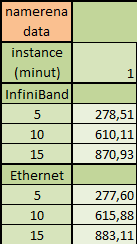
\includegraphics[width=3cm]{sekvencni.png}
  \caption{namerena data pro jeden uzel}
\end{figure}

\section{Popis paralelniho algoritmu a jeho implementace v MPI}
Zakladem paralelniho algoritmu je sekvencni algoritmus. S tim rozdilem, ze stavovy prostor se disjunktne rozdeli mezi vice procesoru, ktere ho samostatne zpracovaji. Kvuli omezujicim podminkam algoritmu DFS-BB si procesory mezi sebou posilaji nalezena nova nejlepsi reseni. Jednotlive procesory maji svuj vlastni lokalni zasobnik a pouziva se dynamicke vyvazovani vypocetni zateze (load balancing). Vyvazovani zateze je implementovano pomoci 2 algoritmu: algoritmu pro deleni zasobniku (ADZ) a algoritmu pro hledani darce (AHD), kterymi necinny procesor s prazdnym lokalnim zasobnikem (stav I=idle) ziskava praci od vhodneho darce, coz je aktivni procesor s neprazdnym zasobnikem (stav A=active), jehoz zasobnik odpovida dostatecne velkemu stavovemu podprostoru. Procesor si o praci zada procesor s cislem o jedno vetsi, pokud ten praci nema, zvysi se citac o jednicku, takto cyklicky zada procesory dokud neobdrzi praci nebo pozadavek na ukonceni. Na pocatku procesor P1 zna pocet procesoru p, na kterych se uloha bude resit. Provede dostatecny pocet expanzi pocatecniho stavu, rozdeli svuj zasobnik na p casti a rozesle jednotlive casti ostatnim procesorum. Vsechny procesory zacnou prohledavat svuj prideleny podprostor a pritom realizuji programovou smycku naznacenou na tomto obrazku.\\

\begin{figure}
  \centering
  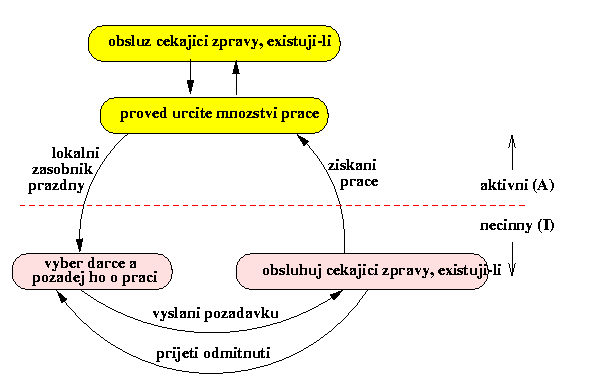
\includegraphics[width=10cm]{CZstatediagram.png}
  \caption{sekvencni}
\end{figure}

Aktivni procesor, ktery vycerpa svuj prideleny dil prace, se stane necinny a pomoci algoritmu pro hledani darce AHD vybere darce a posle mu zadost o praci. Pokud mu darce praci posle, prepne se zpet do stavu aktivni. Pokud se mu vrati odmitnuti, vse se opakuje. Procesor ve stavu necinny musi take periodicky kontrolovat, zda nema ve fronte zadosti o praci, na ktere odpovida odmitnutim, nebo zpravy o nalezeni reseni jinym procesorem. V pripade, ze se jedna o optimalni reseni, jsou to v podstate zadosti o ukonceni vypoctu. Aktivni procesor provadi fixni objem prace nad lokalnim zasobnikem (expanduje urcity dany pocet stavu na lokalnim zasobniku) a pak kontroluje frontu zprav. V te mohou byt zadosti o praci, informace o nalezeni reseni jinym procesorem a zadosti o ukonceni vypoctu. Aktivni procesor zpracovava zadosti o praci nasledujicim zpusobem: Pokud je velikost lokalniho zasobniku vetsi nez nastavena minimalni mez, tak se zasobnik rozdeli na polovinu a jedna cast se zasle zadateli o praci. Pokud neni, tak procesor pozadavek odmitne.

\section{Analyza slozitosti paralelniho reseni}

\subsection{Analyza sekvencniho reseni}
Slozitost sekvencniho reseni lze rozdelit na dve casti. Nejprve na to, kolik stav; se projde, cili jak je velky stavovy prostor a pro kazdy stav se pak jeste provadi algoritmus BFS pro testovani bipartitnosti.
Orezavani algoritmem Branch and Bound se neda odhadnout, proto ho neuvazujeme. Vyska stromu stavoveho prostoru odpovida poctu hran. V kazdem kroku jednu hranu bud odeberu, nebo necham. \\

Pocet prohledavanych stavu je tedy:\\

\begin{math}
\sum_{i = 0}^{|E|} 2^i = 2^{|E|} + 2^{|E|-1} + ... + 2^0 = O(2^{|E|})\\
\end{math}

Test bipartitnosti se provadi prochazenim do sirky. Slozitost tohoto alogirtmus je :\\

\begin{math}
O(|E| + |V|)\\
\end{math}

Celkova slozitost je tedy:\\

\begin{math}
SU(|E|, |V|) = O(|E| + |V|) \times O(2^{|E|}) = O(2^{|E|} \times (|E| + |V|))\\
\end{math}


\subsection{Analyza paralelniho reseni}
Pri paralelnim algoritmu se nejprve expanduje prvnich p stavu, ktere se rozeslou, potom si p procesoru rozdeli stejnou praci, jakou mel sekvencni algoritmus. Toto tvori vypocetni slozku slozitosti. Vedle te jeste musime zapocist slozku komunikacni, ktera vyjadruje komunikac mezi procesory a predavani prace. Tato slozka je uzce zavisla na rovnomernem rozdeleni prace a poloze hledaneho reseni ve stavovem prostoru. Konkretne tuto slozku tedy vyjadrit nemuzeme, nicmene rozhodne neni zanedbatelna, proto ji ve vzorci uvadime symbolicky.\\

Paralelni cas tedy je:\\

\begin{math}
T(|E|,|V|,p) = T{_{v}}(|E|,|V|,p) + T{_{k}}(|E|, |V|,p) =  O(p + \frac{2^{|E|} \times (|E| + |V|)}{p}) + T{_{k}}(|E|,|V|,p)\\
\end{math}

Teoreticka paralelni� cena:\\ 

\begin{math}
C(|E|,|V|,p) = p*T(|E|,|V|,p) =  O(p^2 + (2^{|E|} \times (|E| + |V|)) + T{_{k}}(|E|,|V|,p) \times p\\
\end{math}

Efektivnost:\\

\begin{math}
E(|E|,|V|,p) = \frac{SU(|E|,|V|)}{C(|E|,|V|,p)} = \frac{O(2^{|E|} \times (|E| + |V|)} { O(p^2 + (2^{|E|} \times (|E| + |V|))) + T{_{k}}(|E|,|V|,p) \times p}\\
\end{math}

A zrychleni:\\

\begin{math}
S(|E|,|V|,p) = \frac{SU(|E|,|V|)}{T(|E|,|V|,p)} =  \frac{ O(2^{|E|} \times (|E| + |V|))}{O(p + \frac{2^{|E|} \times (|E| + |V|)}{p}) + T{_{k}}(|E|,|V|,p)} =O(p + \frac{2^{|E|} \times (|E| + |V|)}{p}) + T{_{k}}(|E|,|V|,p)\\
\end{math}

\section{Namerene vysledky a vyhodnoceni}
Z namerenych dat (Figure 3 a 4) je videt, ze namerene casy pro site InfiniBand a Ethernet jsou temer stejne, lisi se v radu par sekund. Vyssi casy jsou prevazne u site Ethernet. S ohlednutim na mozne spozdeni, kter� nemusi vzniknout primo algoritmem, lze rici, ze namerene casy jsou pro obe site stejne. To znamena, ze se neprenasi velke mnozstvi zprav, ktere by algoritmus zpomalovaly.

Z grafu, znazornujici zrychleni (Figure 5 a 6) je videt, ze je na zaklade namerenych dat podobne pro obe site. Nejlepsi rovnomerne zrychleni pro zvolene instance se zda byt pro 12 vypocetnich uzlu.

\subsection{Vyhodnoceni}
V teto uloze jsem nejdrive implementovali sekvencni algoritmus pro hledani bipartitniho podgrafu. Nasledne jsme implementovali paralelni reseni. Toto reseni jsme otestovali na datech ziskanych ze sekvencniho mereni, kde instance bezeli 5, 10 a 15 minut. Tyto instance jsme otestovali na paralelnim algoritmu. Z vyslednych grafu lze rici, ze se algoritmus chova spravne a s poctem vypocetnich uzlu klesa vypocetni cas.

\begin{figure}
  \centering
  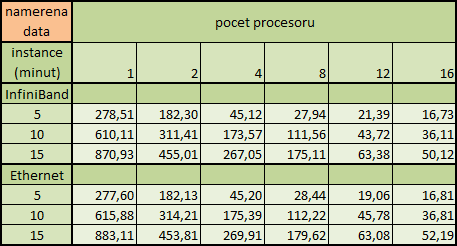
\includegraphics[width=10cm]{namerena_data.png}
  \caption{tabulka namerenych vysledku}
\end{figure}

\begin{figure}
  \centering
  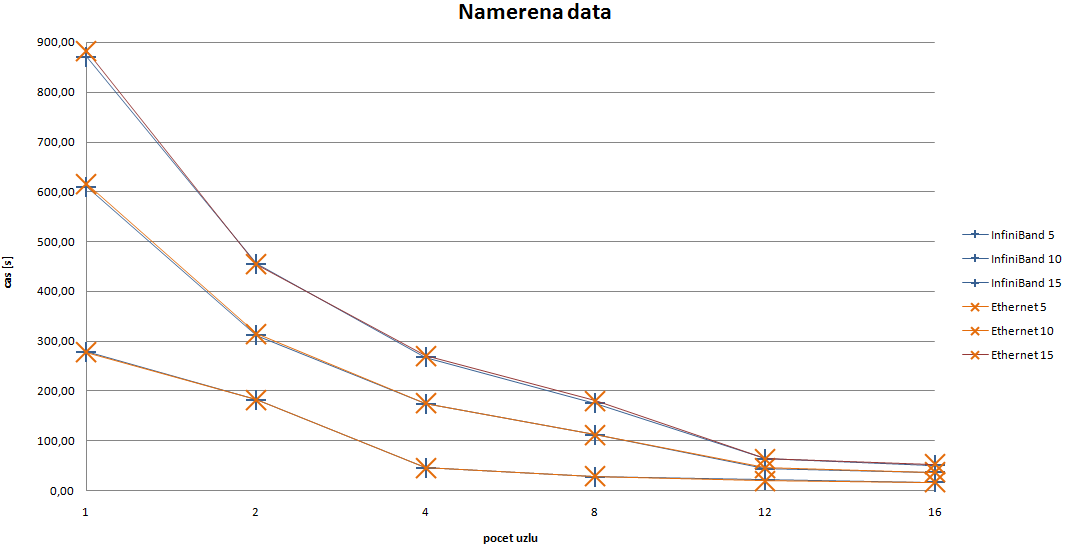
\includegraphics[width=15cm]{namerena_data_graf.png}
  \caption{graf namerenych vysledku}
\end{figure}

\begin{figure}
  \centering
  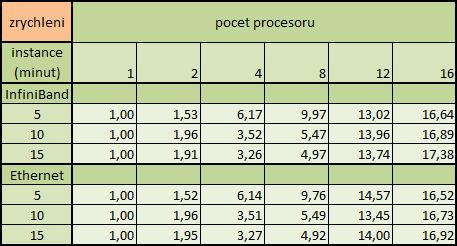
\includegraphics[width=10cm]{zrychleni.png}
  \caption{tabulka zrychleni}
\end{figure}

\begin{figure}
  \centering
  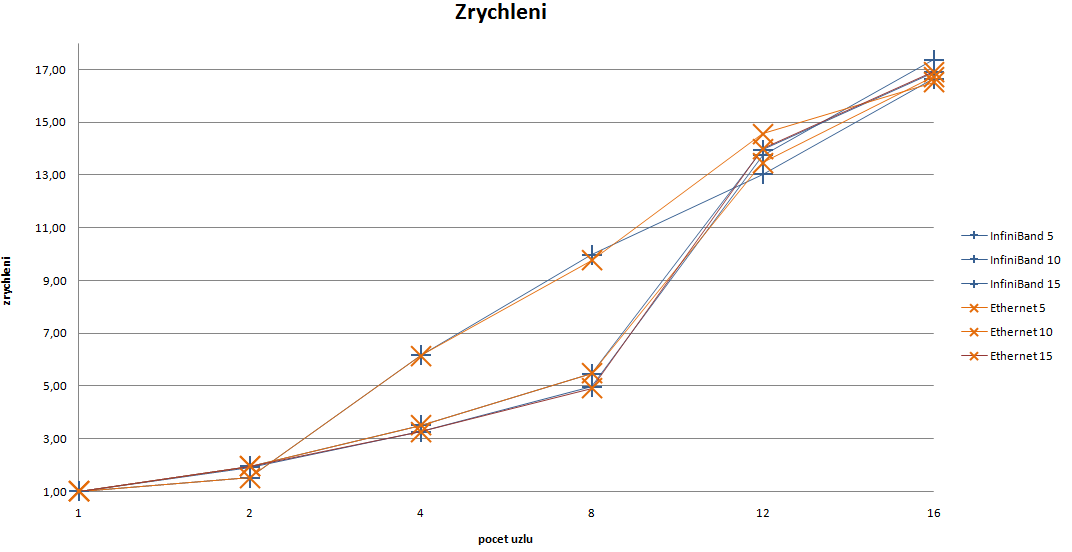
\includegraphics[width=15cm]{zrychleni_graf.png}
  \caption{graf zrychleni}
\end{figure}

\end{document}








